\documentclass[letterpaper, 12pt]{article}
\usepackage[letterpaper, top=2.5cm, bottom=2.5cm, left=3cm, right=3cm]{geometry} %margenes
\usepackage[backend=biber]{biblatex}\addbibresource{bibliografia.bib} %manejo de bibliografía (BORRAR SI NO ES NECESARIO)
\usepackage[utf8]{inputenc} %manejo de caracteres especiales
\usepackage[spanish]{babel} %manejo de encabezados de inglés a español
\usepackage{fancyhdr} %formato de los encabezados de página
\usepackage{ragged2e} %alineado real justficado
\usepackage{graphicx} %manejo de imagenes
\usepackage{amsmath} %manejo de notación matemática
\usepackage{mathtools} %manejo de notación matemática
\usepackage{blindtext} %texto de relleno
\usepackage{amssymb} %manejo de simbología
\usepackage{float} %centrado de imaene
\usepackage{hyperref} %manejo de enlaces e hipervínculos

\hypersetup{
  colorlinks   = true, %Colours links instead of ugly boxes
  urlcolor     = blue, %Colour for external hyperlinks
  linkcolor    = blue, %Colour of internal links
  citecolor   = red %Colour of citations
}

\pagestyle{fancy}
\fancyhf{}
\rfoot{\thepage}

\nocite{*}

\begin{document}
    
    %PORTADA
    \begin{titlepage}
        \begin{figure}[ht]
            \centering
            
\includegraphics[width=15cm]{logosITT.png}
        \end{figure}
        \centering
        {\scshape\LARGE Tecnológico Nacional de México\\Instituto Tecnológico de Tijuana\par}
        \vspace{1cm}
        {\scshape\Large Simulación\par}
        \vspace{1cm}
        {\scshape\Large Unidad 1\par}
        \vspace{1.5cm}
        {\huge\bfseries Estructura y etapas de un estudio de Simulación\par}
        \vspace{2cm}
        {\Large\itshape C. Abraham Jhared Flores Azcona\\19211640\par}
        \vfill
        Profesor: Ing. Diego Saul Vasquez Rios\par
    
        \vfill

        {\large \today}
    \end{titlepage}

    %cuerpo
    \newpage
    \begin{justify}
        \setcounter{page}{1}
        \thispagestyle{fancy}
        \lhead{\textbf{Estructura y etapas de un estudio de Simulación}}
        \section*{Definición del Sistema}
        \justify
        En este paso se envuelve el identificar los componentes del sistema a modelar y las mediciones de rendimiento a ser analizadas. Generalmente
        los sistemas son complejos, por ello la definición del sistema requiere un simulador experimentado que puede encontrar el nivel apropiado de detalle y flexibilidad.
        \section*{Formulación del Modelo}
        \justify
        Es una técnica constructiva en la investigación de operaciones usado para construir la arquitectura matemática de problemas mientras se persigue una función objetivo en las operaciones
        de cualquier organización. Las variables de desición, función objetivo, restricciones y parámetros que son componentes de la función objetivo las cuales constituyen el modelo en Investigación de Operaciones.
        \\\newline
        Entender como funciona el sistema de estudio actual y determinar los requerimientos básicos del modelo son necesarios en desarrollar el modelo correcto. Al crear un diagrama de flújo del como opera el sistema facilita
        la comprensión de como las variables están involucradas como interactuan.
        \section*{Recolección de Datos}
        \justify
        Después de la formulación del modelo, se determina el tipo de dato a recolectar. Luego se procede a recolectar datos nuevos ú existentes. Estos se acomodan a distribuciones teóricas. 
        \\\newline
        A grandes rasgos la recolección se define como el proceso de recolectar, medir y analizar de manera certera por investigación usando técnicas estándares. Su recolección depende del campo de estudio y de la información requerida.
        \section*{Implementación del Modelo en la computadora}
        \justify
        Simple y sencillo. El modelo teórico se traslada a un lenguaje de programación. La opción depende de lo que se necesite: si se requiere eficiencia por calculos complejos se puede usar C, si buscamos una experiencia sencilla con la simulación
        se puede preferir el usar programas de simulación como Arena.
        \section*{Validación}
        \justify
        Se incluye también a la verificación en este paso. El proceso de verificación asegura que el modelo se comporte a lo esperado, esto se logra con el debugging o con la animación. La validación asegura que no exista alguna diferencia significativa entre el modelo
        y el sistema real y que el modelo refleja la realidad. La validación se puede lograr por el análisis estadístico.
        \\\newline
        Un proceso típico de validación consiste de los aspectoss siguientes:
        \begin{itemize}
            \item Verificar que la entrada y salida del modelo esté limpia. Sumandose que estén los controles suficientes para lidiar con problemas de calidad de datos así como exparsir entradas faltantes.
            \item Revisar que la entrada del modelo sea estable y representativa.
            \item Verificar la implementación del modelo, lo que significa que estamos probando la expectativa del modelo.
            \item Comparar el modelo conn alternativas para analizar el impacto de las presunciones del modelo cambiante.
            \item Analizar la estabilidad del modelo así como su robustéz del procedimiento de calibración.
        \end{itemize}
        \section*{Experimentación}
        \justify
        Realizamos la próctica del modelo en acción. Todo resultado relevante se almacena para su posterior análisis e interpretación.
        \section*{Interpretación}
        \justify
        Se hacen los análisis correspondientes de los datos recabados en el paso anterior. Despues de curar los datos se procede a su interpretación para que se conviertan en información útil para obtener las conclusiones.
        \section*{Documentación}
        \justify
        Correponde simplemente a escribir el reporte y/o presentación correspondiente a la simulación.
        
        \newpage
        \section*{Diagrama alusivo}
        \begin{figure}[H]
            \centering
            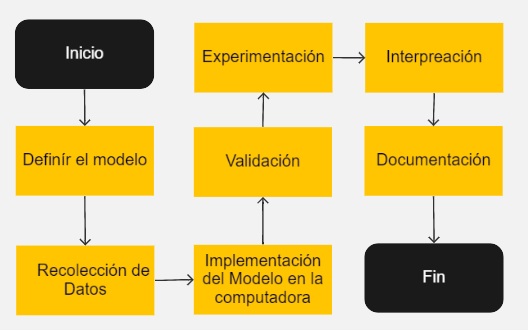
\includegraphics[width=10cm,height=8cm]{diagrama.PNG}
            \caption{Diagrama alusivo a las etapas de un estudio de simulación.}
        \end{figure}

    \end{justify}

    %bibliografía
        \thispagestyle{empty}
        \printbibliography
\end{document}